\documentclass[12pt,a4paper,onecolumn]{article}
\usepackage[utf8]{inputenc}
\usepackage[T1]{fontenc}
\usepackage[french]{babel}

% ------------------------- Color table ----------------------------------------
\usepackage{multirow}
\usepackage[table]{xcolor}
\definecolor{maroon}{cmyk}{0,0.87,0.68,0.32}
% ------------------------------------------------------------------------------

\usepackage{amscd}
\usepackage{amsthm}
\usepackage{physics}
\usepackage[left=2.2cm,right=2.2cm,top=2cm,bottom=2cm]{geometry}
\usepackage{textcomp,gensymb} %pour le °C, et textcomp pour éviter les warning
\usepackage{graphicx} %pour les images
\usepackage{caption}
\usepackage{subcaption}
\usepackage[colorlinks=true,
	breaklinks=true,
	citecolor=blue,
	linkcolor=blue,
	urlcolor=blue]{hyperref} % pour insérer des liens
\usepackage{epstopdf} %converting to PDF
\usepackage[export]{adjustbox} %for large figures

\usepackage{array}
\usepackage{dsfont}% indicatrice : \mathds{1}


% -------------------------- Mathematics ---------------------------------------
\graphicspath{{images/}} % For the images path
% ------------------------------------------------------------------------------

% -------------------------- Mathematics ---------------------------------------
\usepackage{mathrsfs, amsmath, amsfonts, amssymb}
\usepackage{bm}
\usepackage{mathtools}
\usepackage[Symbol]{upgreek} % For pi \uppi different from /pi
\newcommand{\R}{\mathbb{R}} % For Real space
% ------------------------------------------------------------------------------


% -------------------------- Code format ---------------------------------------
\usepackage[numbered,framed]{matlab-prettifier}
\lstset{
	style              = Matlab-editor,
	basicstyle         = \mlttfamily,
	escapechar         = '',
	mlshowsectionrules = true,
}
% ------------------------------------------------------------------------------

% ------------------------- Blbiographie --------------------------------------
% \usepackage[backend=biber, style=science]{biblatex}
% \addbibresource{biblio.bib}
% ------------------------------------------------------------------------------


\setcounter{tocdepth}{4} %Count paragraph
\setcounter{secnumdepth}{4} %Count paragraph
\usepackage{float}

\usepackage{graphicx} % for graphicspath
% \graphicspath{{../images/}}

\usepackage{array,tabularx}
\newcolumntype{L}[1]{>{\raggedright\let\newline\\\arraybackslash\hspace{0pt}}m{#1}}
\newcolumntype{C}[1]{>{\centering\let\newline\\\arraybackslash\hspace{0pt}}m{#1}}
\newcolumntype{R}[1]{>{\raggedleft\let\newline\\\arraybackslash\hspace{0pt}}m{#1}}

\newcommand{\assignmenttitle}{}
\newcommand{\studentname}{}
\newcommand{\email}{}
\newcommand{\schoolyear}{2017/2018}


\title{
\normalfont \normalsize 
\textsc{Object recognition and computer vision, Master MVA, \schoolyear} \\
[10pt] 
\rule{\linewidth}{0.5pt} \\[6pt] 
\huge \assignmenttitle \\
\rule{\linewidth}{2pt}  \\[10pt]
}

\author{\studentname}

\date{\small\email}

\newcommand{\question}[1]{\subsubsection*{#1}}

\setlist[enumerate]{topsep=0pt,itemsep=-1ex,partopsep=1ex,parsep=1ex,label=(\roman*)}

\graphicspath{{images/}}

\newcommand{\labelnotempty}[1]{
\def\temp{#1}\ifx\temp\empty
\else
    \label{#1}
\fi
}
% single figure
\newcommand{\singlefig}[4]{
\begin{figure}[ht!]
        \centering
        \includegraphics[width={#2}\columnwidth]{#1}
        \caption{#3}
        \labelnotempty{#4}
\end{figure}}

\newcommand{\subfig}[4]{
\includegraphics[width={#2}\columnwidth]{#1}
\caption{#3}
\labelnotempty{#4}
}

% double figure
\newcommand{\doublefig}[4]{
\begin{figure}[ht!]
    \centering
    \begin{subfigure}[t]{0.45\columnwidth}
        \centering
    #1
    \end{subfigure}
    ~
    \begin{subfigure}[t]{0.45\columnwidth}
        \centering
    #2
    \end{subfigure}
    \caption{#3}
    \labelnotempty{#4}
\end{figure}}

% triple figure
\newcommand{\triplefig}[5]{
\begin{figure}[ht!]
    \centering
    \begin{subfigure}[t]{0.30\columnwidth}
        \centering
    #1
    \end{subfigure}
    ~
    \begin{subfigure}[t]{0.30\columnwidth}
        \centering
    #2
    \end{subfigure}
    ~
    \begin{subfigure}[t]{0.30\columnwidth}
        \centering
    #3
    \end{subfigure}
    \caption{#4}
    \labelnotempty{#5}
\end{figure}}



% ------------------------ General informations --------------------------------
\title{Matrice Fondamentale}
\author{Vincent Matthys}
\graphicspath{{images/}}
% ------------------------------------------------------------------------------


\begin{document}

\begin{tabularx}{0.9\textwidth}{@{} l X r @{} }
	{\textsc{Master MVA}}               &  & \textsc{TP2}       \\
	\textsc{Sub-pixel image processing} &  & {ENS Paris Saclay} \\
\end{tabularx}
\vspace{1.5cm}
\begin{center}

	\rule[11pt]{5cm}{0.5pt}

	\textbf{\LARGE \textsc{Compte-rendu TP3}}
	\vspace{0.5cm}

	Vincent Matthys

	vincent.matthys@ens-paris-saclay.fr

	\rule{5cm}{0.5pt}

	\vspace{1.5cm}
\end{center}

\section{Exercice 6}

\begin{figure}[H]
	\centering
	\begin{subfigure}[b]{\textwidth}
		\centering
		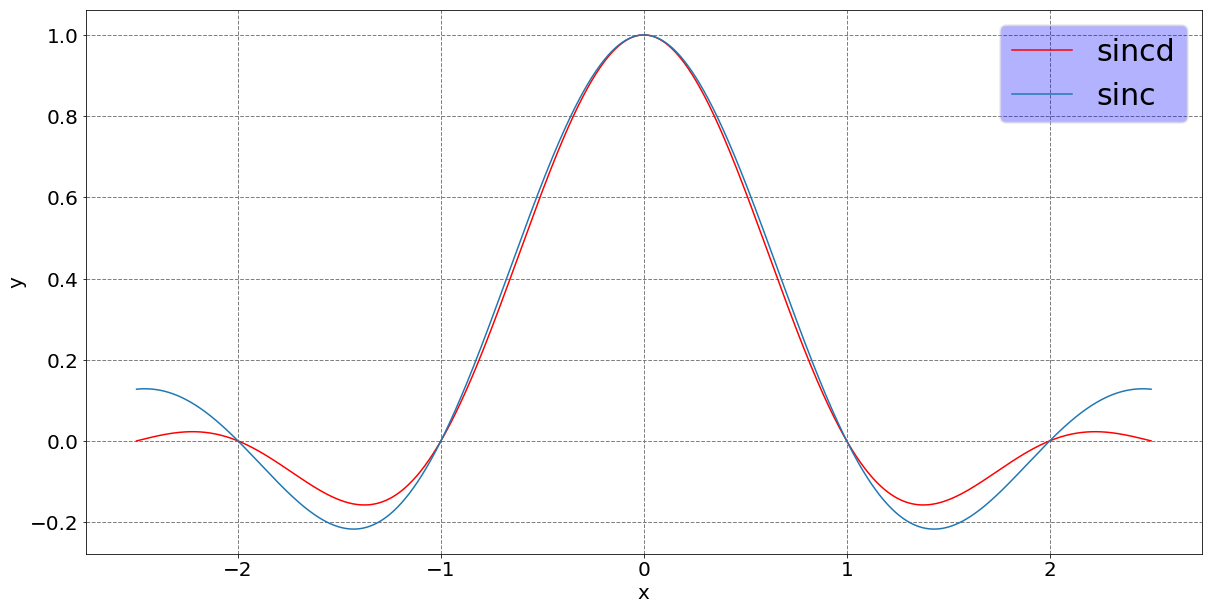
\includegraphics[height = 0.25\textheight]{6_5}
		\subcaption{Pour \(N = 5\)}
		\label{fig_6_5}
	\end{subfigure}
	\begin{subfigure}[b]{\textwidth}
		\centering
		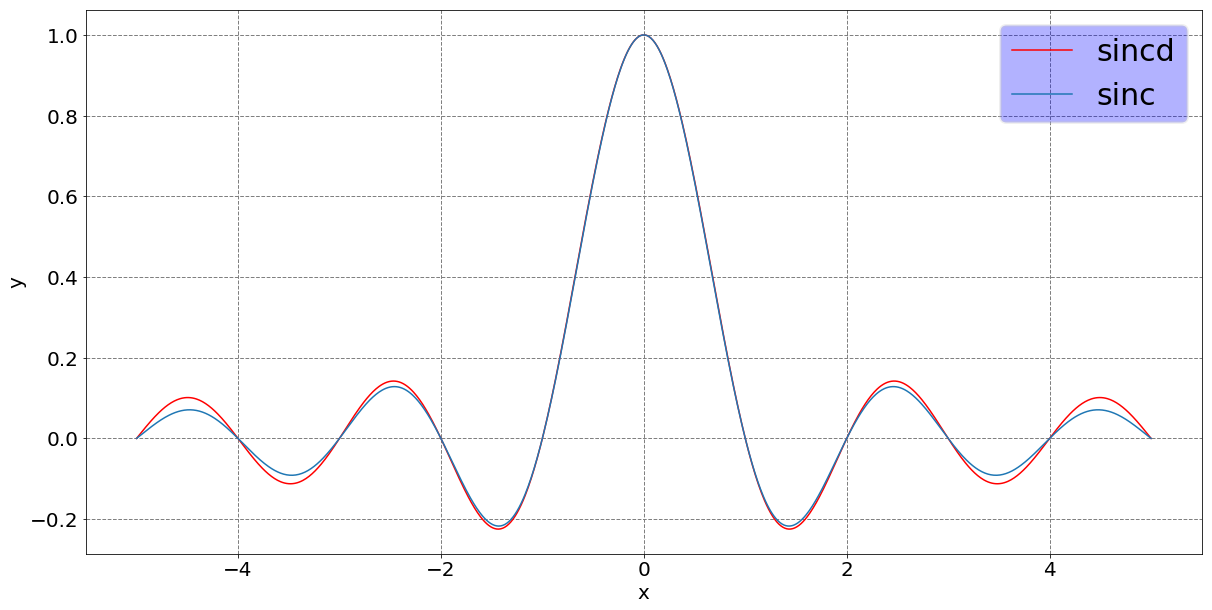
\includegraphics[height = 0.25\textheight]{6_10}
		\subcaption{Pour \(N = 10\)}
		\label{fig_6_10}
	\end{subfigure}
	\begin{subfigure}[b]{\textwidth}
		\centering
		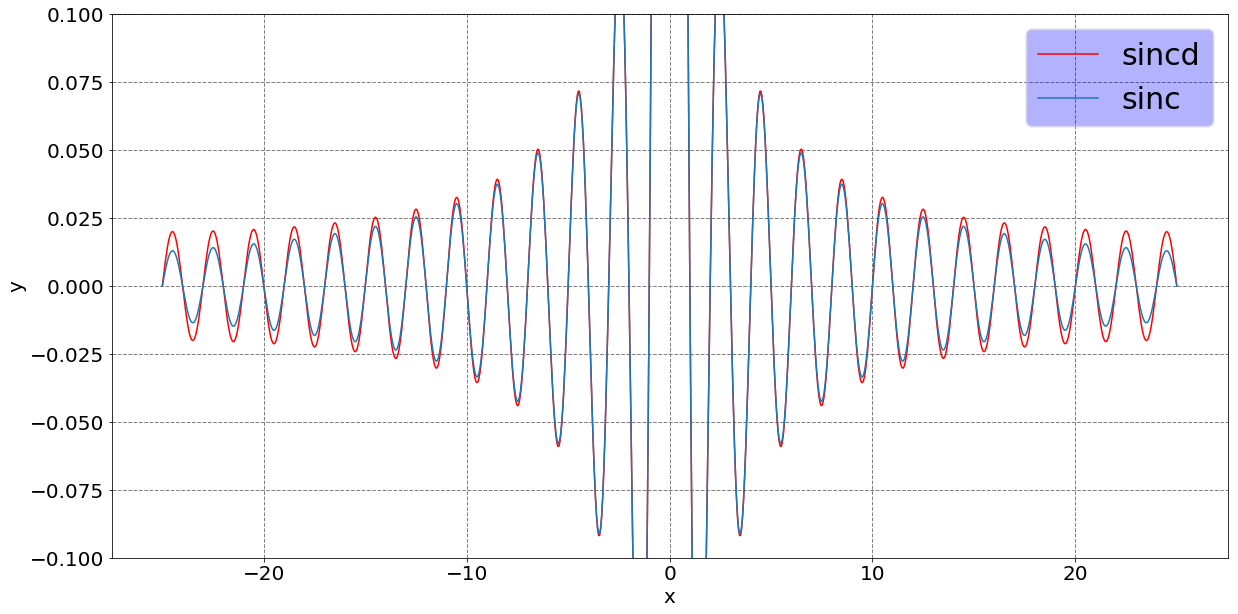
\includegraphics[height = 0.25\textheight]{6_50}
		\subcaption{Pour \(N = 50\)}
		\label{fig_6_50}
	\end{subfigure}
	\caption{Représentation graphique de la convergence du \(sincd_N\) et du \(sinc\), sur \([-N/2, N/2]\)}
	\label{fig_6}
\end{figure}

En figure~\ref{fig_6} sont représentés le \(sinc\) et le \(sincd_N\), pour différentes valeurs de \(N\) pour \(x \in[-N/2, N/2]\). On constate que, pour chaque valeur entière, on a bien égalité, et que, pour N assez grand, les différences sont minimes.

\section{Exercice 7}

\begin{figure}[H]
	\centering
	\begin{subfigure}[b]{\textwidth}
		\centering
		\begin{lstlisting}[frame = none, numbers = none]
		u = double(imread('lena.pgm'));
		\end{lstlisting}
		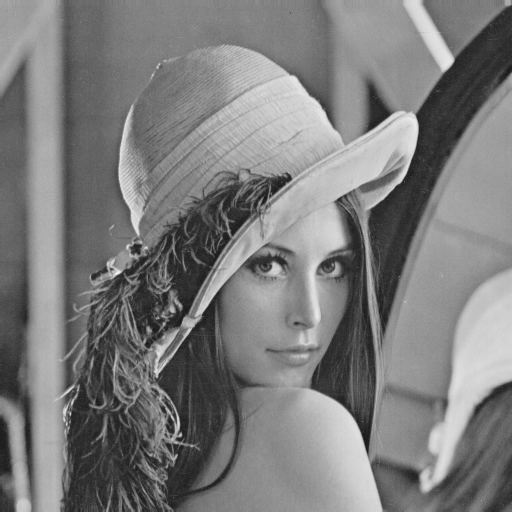
\includegraphics[scale = 1, height = 0.3\textheight]{lena.png}
		\subcaption{Image lena}
	\end{subfigure}
	\vspace{2cm}
	\begin{subfigure}[b]{\textwidth}
		\centering
		\begin{lstlisting}[frame=none, numbers = none]
		f = fft2(u);
		imshow(f, 'InitialMagnification', 100);
		\end{lstlisting}
		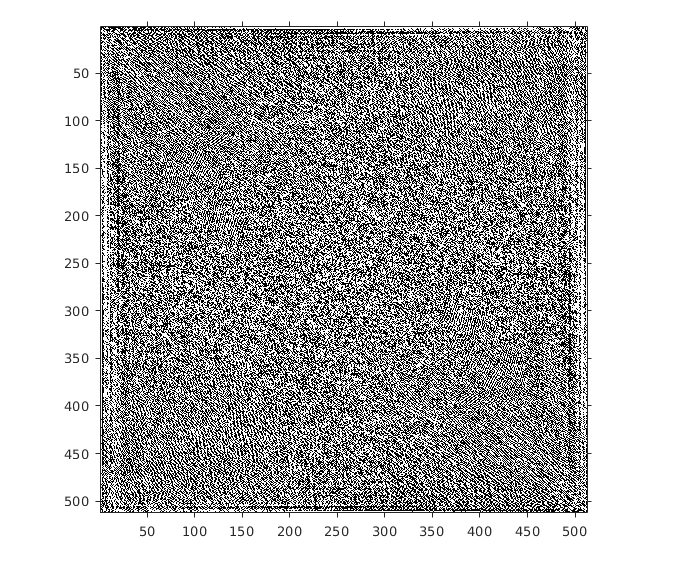
\includegraphics[scale = 1, height = 0.3\textheight]{7_1}
		\subcaption{Partie réelle de la transformée de Fourier de lena}
	\end{subfigure}
	\caption{Partie réelle de la transformée de Fourier de Lena}
	\label{7_1}
\end{figure}

En figure~\ref{7_1}, on demande à Matlab d'afficher en niveaux de gris une matrice complexe, résultant en un message d'erreur \textit{Warning: Displaying real part of complex input.}. On observe donc uniquement la partie réelle de la transformée de Fourier.

\begin{figure}[H]
	\centering
	\begin{subfigure}[b]{\textwidth}
		\centering
		\begin{lstlisting}[frame = none, numbers = none]
		imshow(abs(f));
		\end{lstlisting}
		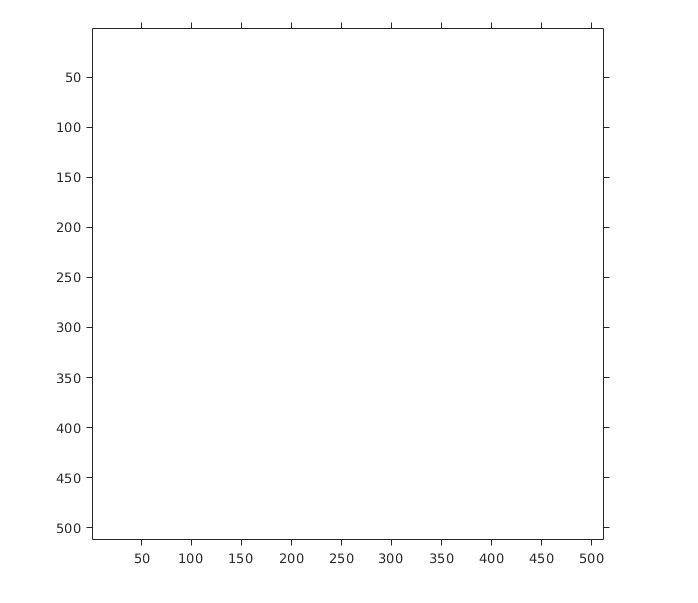
\includegraphics[scale = 1, height = 0.3\textheight]{7_21}
		\subcaption{Sans l'option [] de imshow}
		\label{7_21}
	\end{subfigure}
	\vspace{2cm}
	\begin{subfigure}[b]{\textwidth}
		\centering
		\begin{lstlisting}[frame=none, numbers = none]
		imshow(abs(f),[]);
		\end{lstlisting}
		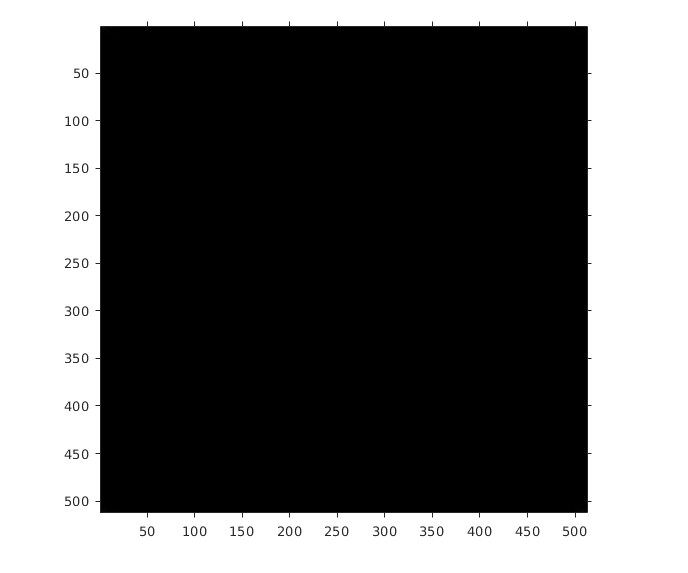
\includegraphics[scale = 1, height = 0.3\textheight]{7_22}
		\subcaption{Avec l'option [ ] de imshow}
		\label{7_22}
	\end{subfigure}
	\caption{Représentations du module de la transformée de Fourier}
	\label{7_2}
\end{figure}

En figure~\ref{7_2}, la commande~\ref{7_21} est équivalent à :
\begin{lstlisting}[numbers = none]
imshow(abs(f) > 1);
\end{lstlisting}
et on n'obtient que des pixels blancs, puisque imshow, quand on lui présente un double (ce qui est le type de abs(f)), représente en noir les valeurs à 0, en blanc les valeurs à 1, et en niveaux de gris les valeurs entre ces bornes. Or, on vérifie que abs(1) > 1 ne contient que des 1. En revance, avec l'option [ ], on rescale \(abs(f) \in [0, 1]\), avec la plus grande valeur en blanc, et la plus faible en noire. Or, la répartition des valeurs est très asymétrique, et on ne représente quasiment que du noir. On peut s'en convaincre en tracant le logarithme de cette image, qui donne la figure~\ref{7_33}.

\begin{figure}[H]
	\centering
	\begin{lstlisting}[frame=none, numbers = none]
	imshow(log(abs(f)),[]);
	\end{lstlisting}
	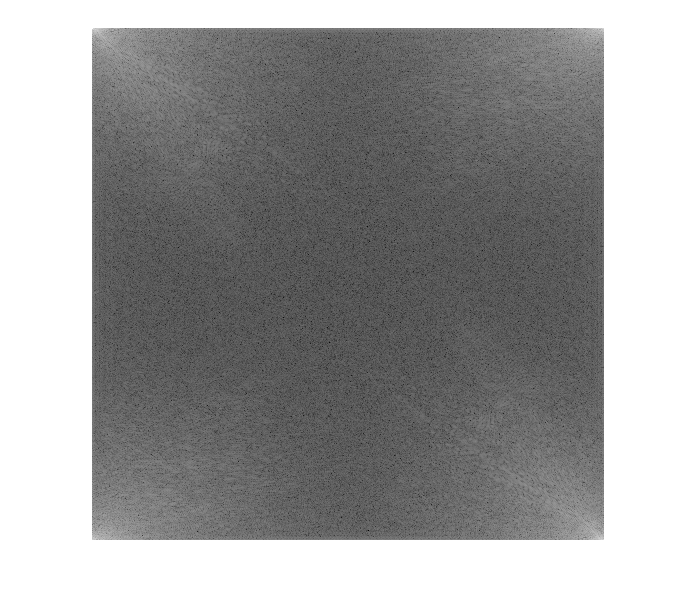
\includegraphics[height = 0.3\textheight]{7_33}
	\caption{Logarithme de la figure~\ref{7_22}}
	\label{7_33}
\end{figure}

En figure~\ref{7_3}, on sature \(1~\%\) des valeurs extremales du module de la transformée, et on redistribue linéairement les valeurs restantes sur tous les niveaux de gris. C'est ce que fait la fonction \textit{normsat}. La fonction \textit{fftshift} permet de centrer l'origine des fréquences, passant du coin supérieur gauche en figure~\ref{7_31} au centre en figure~\ref{7_32}.

\begin{figure}[H]
	\centering
	\begin{subfigure}[b]{\textwidth}
		\centering
		\begin{lstlisting}[frame = none, numbers = none]
		imshow(normsat(abs(f),1));
		\end{lstlisting}
		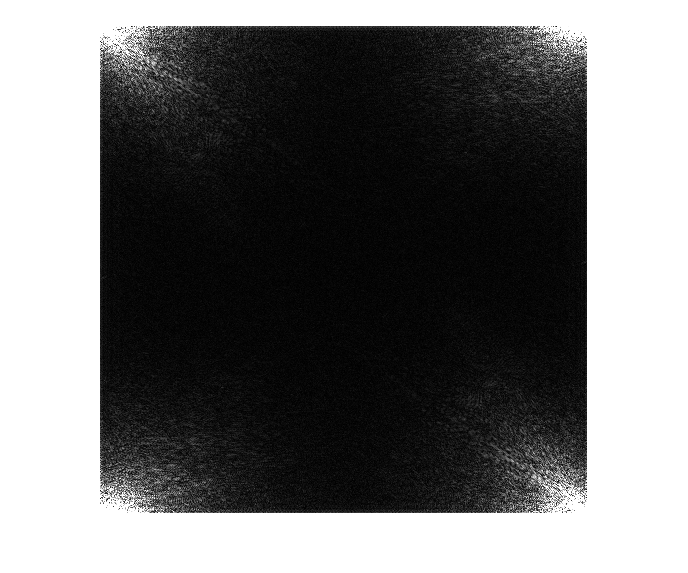
\includegraphics[scale = 1, height = 0.3\textheight]{7_31}
		\subcaption{Avec l'origine des fréquences en haut à gauche de l'image}
		\label{7_31}
	\end{subfigure}
	\vspace{2cm}
	\begin{subfigure}[b]{\textwidth}
		\centering
		\begin{lstlisting}[frame=none, numbers = none]
		imshow(normsat(fftshift(abs(f)),1));
		\end{lstlisting}
		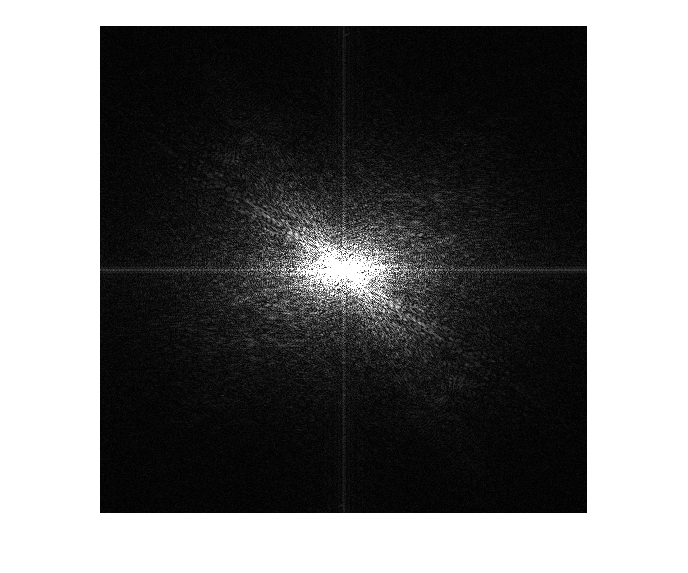
\includegraphics[scale = 1, height = 0.3\textheight]{7_32}
		\subcaption{Avec l'origine des fréquences au milieu de l'image}
		\label{7_32}
	\end{subfigure}
	\caption{Visualisation du module de la transformée de Fourier après saturation à \(1~\%\) des valeurs extremales et mapping linéaire des valeurs restantes en niveau de gris}
	\label{7_3}
\end{figure}

En figure~\ref{7_44} sont présentés les commandes et leur résultat pour visualier efficacement différentes parties d'une transformée de Fourier.

\begin{figure}
	\centering
	\begin{subfigure}[b]{0.45\textwidth}
		\centering
		\begin{lstlisting}[frame = none, numbers = none]
imshow(log(1 +abs(real(fftshift(f)))), [])
		\end{lstlisting}
		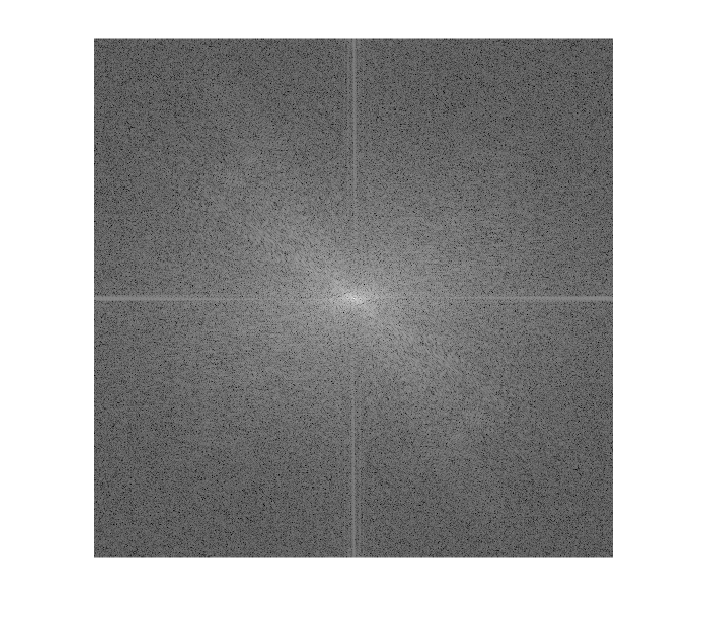
\includegraphics[scale = 1, width = \textwidth]{7_41}
		\subcaption{Logarithme de la partie réelle}
		\label{7_41}
	\end{subfigure}
	\begin{subfigure}[b]{0.45\textwidth}
		\centering
		\begin{lstlisting}[frame = none, numbers = none]
imshow(log(1 +abs(imag(fftshift(f)))), [])
		\end{lstlisting}
		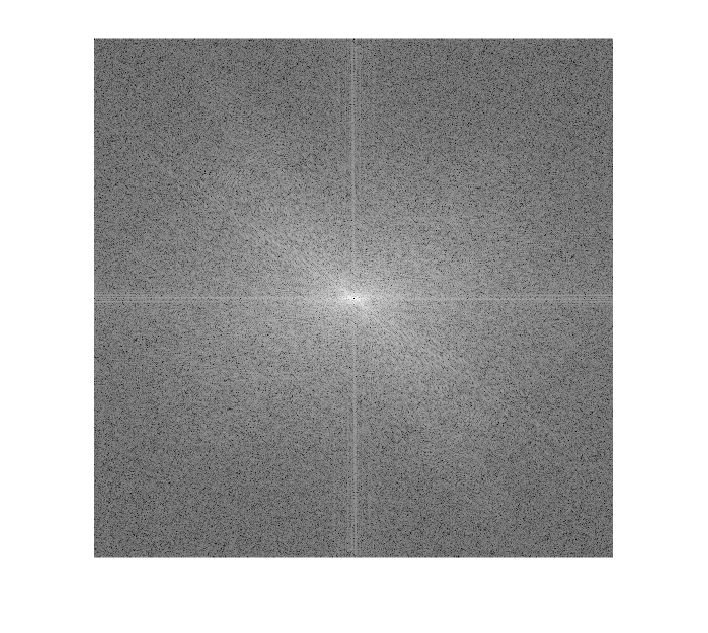
\includegraphics[scale = 1, width = \textwidth]{7_42}
		\subcaption{Logarithme de la partie imaginaire}
		\label{7_42}
	\end{subfigure}
	\begin{subfigure}[b]{0.45\textwidth}
		\centering
		\begin{lstlisting}[frame = none, numbers = none]
imshow(angle(fftshift(f)) + pi, [])
		\end{lstlisting}
		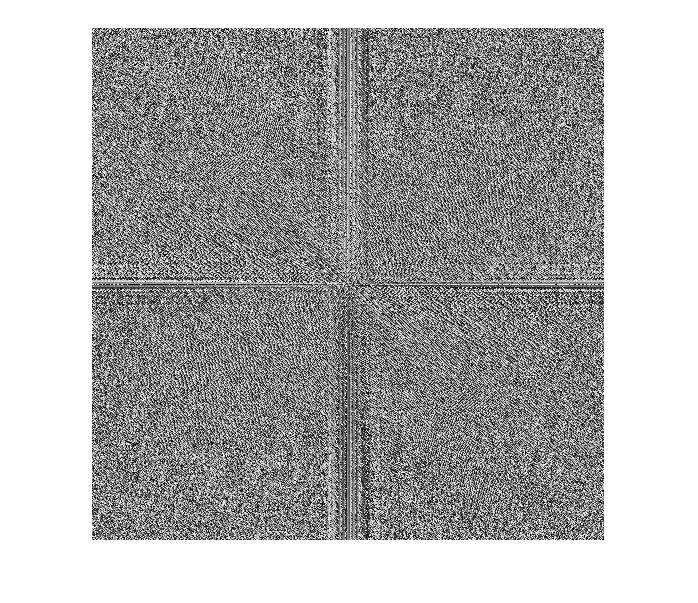
\includegraphics[scale = 1, width = \textwidth]{7_43}
		\subcaption{Phase}
		\label{7_43}
	\end{subfigure}
	\begin{subfigure}[b]{0.45\textwidth}
		\centering
		\begin{lstlisting}[frame = none, numbers = none]
imshow(log(1 +abs(fftshift(f))), [])
		\end{lstlisting}
		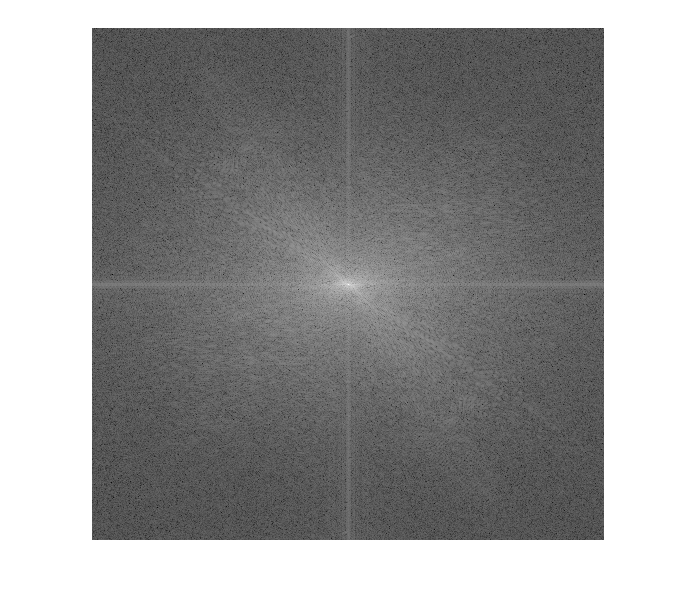
\includegraphics[scale = 1, width = \textwidth]{7_44}
		\subcaption{Logarithme du module}
		\label{7_44}
	\end{subfigure}
	\caption{Visualisation des divers parties d'une transformée de Fourier}
	\label{}
\end{figure}

\clearpage

\section{Exercice 8}

\subsection{Question 1}

\begin{equation}
	\begin{split}
		U &= \sum_{0\le k \le M-1,~0 \le l \le N-1}u(k,l)\sum_{m,n\in \mathbb{Z}}\delta_{(k + mM, l + nN)}\\
		\widehat{U}(\bm{\xi}) &= \sum_{0\le k \le M-1,~0 \le l \le N-1}u(k,l) \int_{\mathbb{R}^2}\sum_{m,n\in \mathbb{Z}}\delta_{(k + mM, l + nN)}(x, y)e^{-ix\xi_x - iy\xi_y}dxdy \\
		\widehat{U}(\bm{\xi}) &= \sum_{0\le k \le M-1,~0 \le l \le N-1}u(k,l) \int_{\mathbb{R}^2}\sum_{m,n\in \mathbb{Z}}\delta_{(mM, nN)}(x - k, y - l)e^{-ix\xi_x - iy\xi_y}dxdy \\
		\widehat{U}(\bm{\xi}) &= \sum_{0\le k \le M-1,~0 \le l \le N-1}u(k,l) e^{-i(k\xi_x + l\xi_y)}\int_{\mathbb{R}^2}\sum_{m,n\in \mathbb{Z}}\delta_{(mM, nN)}(x, y)e^{-ix\xi_x - iy\xi_y}dxdy \\
		\widehat{U}(\bm{\xi}) &= \sum_{0\le k \le M-1,~0 \le l \le N-1}u(k,l) e^{-i(k\xi_x + l\xi_y)}\widehat{\Pi_{M, N}}(\bm{\xi}) \\
		\widehat{U}(\bm{\xi}) &= \sum_{0\le k \le M-1,~0 \le l \le N-1}u(k,l) e^{-i(k\xi_x + l\xi_y)}\frac{2\pi}{M}\frac{2\pi}{N}\Pi_{\frac{2\pi}{M}, \frac{2\pi}{N}}(\bm{\xi}) \\
		\widehat{U}(\bm{\xi}) &= \frac{2\pi}{M}\frac{2\pi}{N}\sum_{p,q\in \mathbb{Z}}\delta_{\frac{2\pi}{M}, \frac{2\pi}{N}}(\bm{\xi})\sum_{0\le k \le M-1,~0 \le l \le N-1}u(k,l) e^{-i(2\pi pk/M + 2\pi lq/N)}\\
		\widehat{U}(\bm{\xi}) &= \frac{2\pi}{M}\frac{2\pi}{N}\sum_{p,q\in \mathbb{Z}}\widehat{u}(p, q) \delta_{\frac{2\pi}{M}, \frac{2\pi}{N}}(\bm{\xi})\\
	\end{split}
	\label{eq_8_1}
\end{equation}

La relation étable en~\eqref{eq_8_1} montre que la tranformée de fourier discrète agit comme si le signal initial était déjà périodique, puisque les coefficients de Fourier sont ceux du signal périodisé.

\subsection{Question 2}

\begin{equation}
	\begin{split}
		\widehat{u}'(p, q) &= \sum_{k = 0}^{M - 1} \times \sum_{l = 0}^{N - 1}e^{-2i\pi pk/M}e^{-2i\pi ql/N}u'(k, l) \\
		&= \sum_{k = 0}^{M - 1} \times \sum_{l = 0}^{N - 1}e^{-2i\pi pk/M}e^{-2i\pi ql/N}\dot{u}(k + k_0, l + l_0)\\
		&= \sum_{k' = k_0}^{k_0 + M - 1} \times \sum_{l' = l_0}^{l_0 + N - 1}e^{-2i\pi p(k' - k_0)/M}e^{-2i\pi q(l'-l_0)/N}\dot{u}(k', l') \\
		&= e^{-2i\pi pk_0/M}e^{-2i\pi ql_0/N}\sum_{k' = k_0}^{k_0 + M - 1} \times \sum_{l' = l_0}^{l_0 + N - 1}e^{-2i\pi pk'/M}e^{-2i\pi ql'/N}\dot{u}(k', l') \\
		&= e^{-2i\pi pk_0/M}e^{-2i\pi ql_0/N}\widehat{u}(p, q)
	\end{split}
	\label{eq_8_2}
\end{equation}

Et on constate donc que les coefficients de Fourier de la translatée périodique sont, en module, identiques aux coefficients de Fourier de l'image, mais avec une phase modifiée qui dépend de la translation.

\subsection{Question 3}

\begin{figure}[H]
	\centering
	\begin{subfigure}[b]{\textwidth}
		\centering
		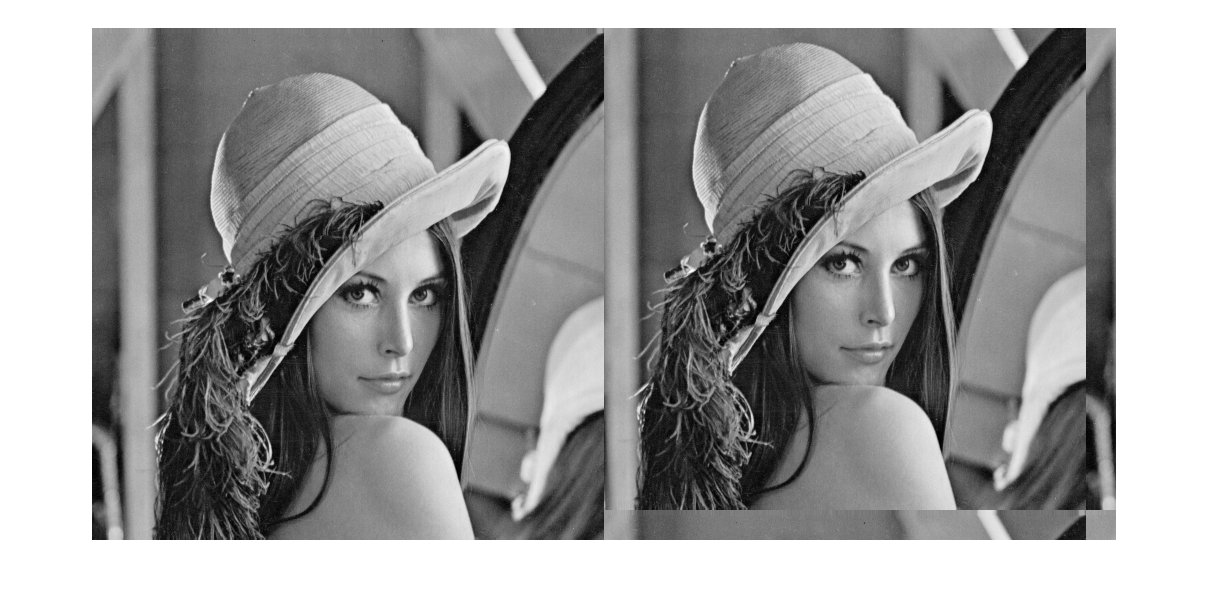
\includegraphics[height = 0.24\textheight]{8_3_images}
		\subcaption{Images initiales}
		\label{8_3_images}
	\end{subfigure}
	\begin{subfigure}[b]{\textwidth}
		\centering
		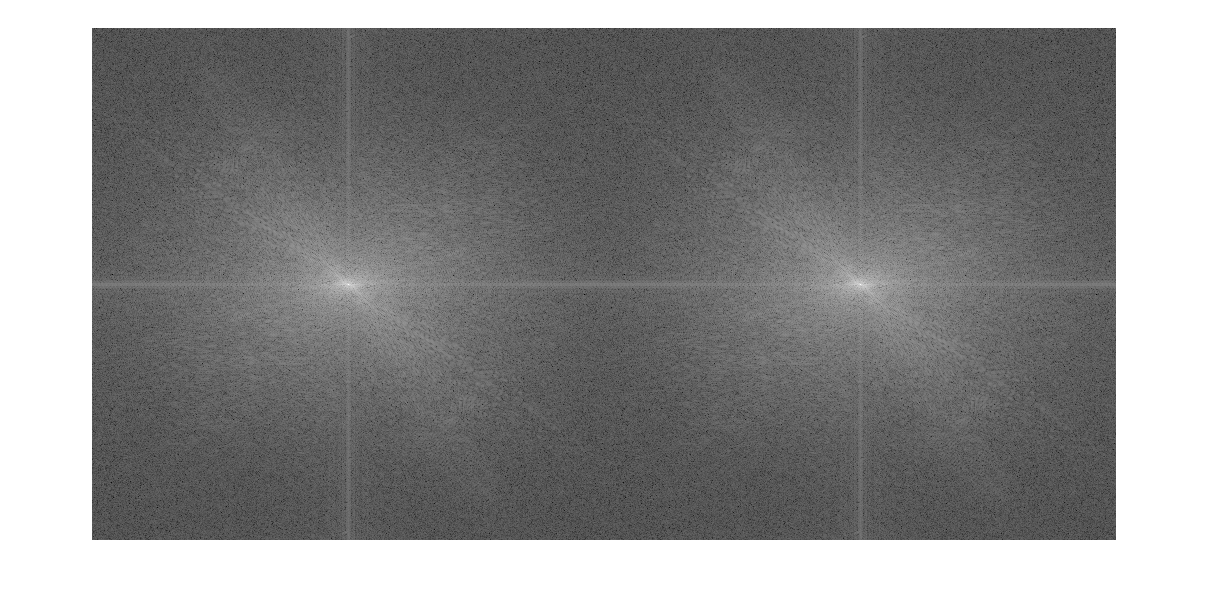
\includegraphics[height = 0.24\textheight]{8_3_mod}
		\subcaption{Visualisation du module de la transformée de Fourier}
		\label{8_3_mod}
	\end{subfigure}
	\begin{subfigure}[b]{\textwidth}
		\centering
		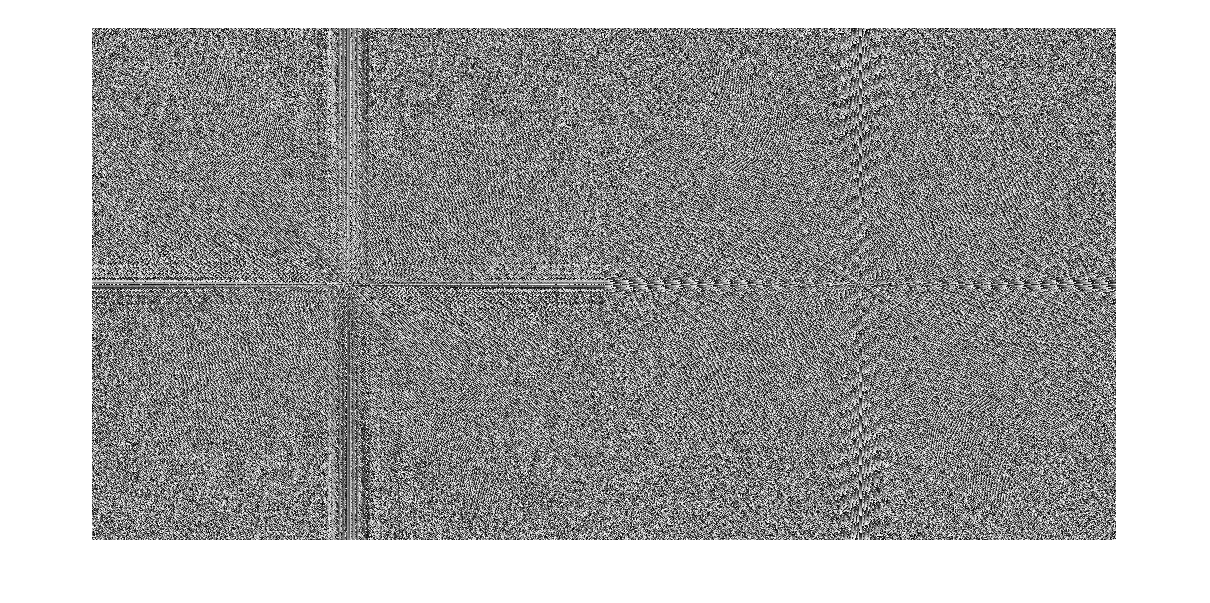
\includegraphics[height = 0.24\textheight]{8_3_phase}
		\subcaption{Visualistion de la phase de la transformée de Fourier}
		\label{8_3_phase}
	\end{subfigure}
	\caption{Effet de la périodisation implicite sur le module et la phase de la transformée de Fourier : translation de lena périodisée.}
	\label{8_3}
\end{figure}

En figure~\ref{8_3}, on présente l'image translatée \textit{lena} après périodisation. On retrouve bien que le module de la transformée de Fourier, visualisée en figure~\ref{8_3_mod} ne varie pas, mais la phase de celle-ci est modifiée, comme présenté en figure~\ref{8_3_phase}. On retrouve effectivement les résultats de la question 2.

\clearpage

\section{Exercice 9}

L'interpolée de Shannon \(v(x,y)\) en fonction de \(\widehat{u}\) s'écrit :

\begin{equation}
	v(x,y) = \frac{1}{MN}\sum_{\mathclap{{|\alpha| \le M/2, |\beta| \le N/2, (p,q) \in \mathbb{Z}}}}\epsilon_M(\alpha)\epsilon_N(\beta)\widehat{u}(\alpha, \beta)  e^{2i\pi(\frac{\alpha x}{M} + \frac{\beta y}{N})}
\end{equation}

avec \(\epsilon_N(p) = 0.5\) si \(|p| = N/2\), donc dans le cas N pair, et 0 sinon

Montrons que :
\begin{equation}
	w(x,y) = \Re\left(\frac{1}{MN}\sum_{\substack{-M/2 \le \alpha < M/2\\ -N/2 \le \beta < N/2}} \widehat{u}(\alpha, \beta) e^{2i\pi(\frac{\alpha x}{M} + \frac{\beta y}{N})} \right)
\end{equation}
définit une interpolation exacte de \(u\).
En effet, on a, pour \((k,l) \in \mathbb{Z}\)

\begin{equation}
	\begin{split}
		w(k,l) &= \Re\left(\frac{1}{MN}\sum_{\substack{-M/2 \le \alpha < M/2\\ -N/2 \le \beta < N/2}}  \widehat{u}(\alpha, \beta) \exp\left(2i\pi(\frac{\alpha k}{M} + \frac{\beta l}{N})\right) \right) \\
		&= \Re\left(\frac{1}{MN}\sum_{\substack{-M/2 \le \alpha < M/2\\ -N/2 \le \beta < N/2}}  \left( \sum_{p, q = 0}^{M-1, N-1}u(p, q)\exp\left(-2i\pi(\frac{\alpha p}{M} + \frac{\beta q}{N})\right)\right) \exp\left(2i\pi(\frac{\alpha k}{M} + \frac{\beta l}{N})\right) \right)\\
		&= \Re\left(\frac{1}{MN} \sum_{p, q = 0}^{M-1, N-1}u(p, q) \left( \sum_{\substack{-M/2 \le \alpha < M/2\\ -N/2 \le \beta < N/2}} \exp\left(2i\pi(\alpha \frac{k - p}{M} + \beta\frac{l-q}{N})\right)\right)\right)\\
		&= \Re\left(\frac{1}{MN} \sum_{p, q = 0}^{M-1, N-1}u(p, q) M\delta(k-p)N\delta(l-q)\right)\\
		&= u(k,l)
	\end{split}
\end{equation}

\section{Exercice 10}

\subsection{Question 1}

\begin{figure}[H]
	\centering
	\begin{subfigure}[b]{\textwidth}
		\centering
		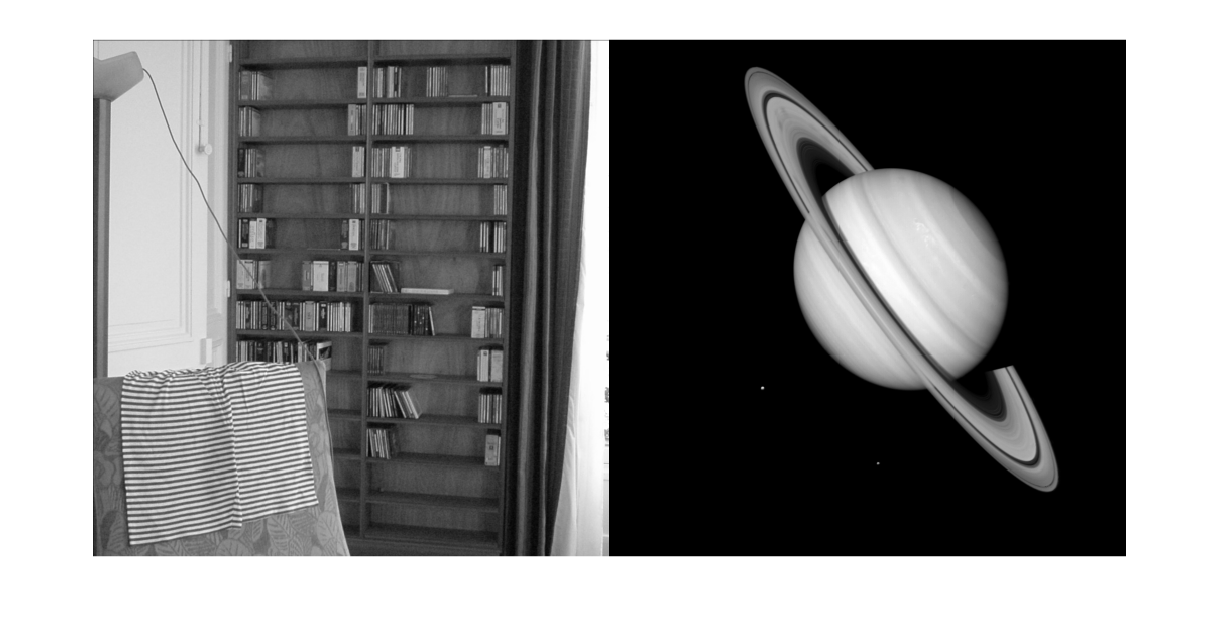
\includegraphics[height = 0.30\textheight]{10_1_11}
		\subcaption{Images initiales}
		\label{10_1_11}
	\end{subfigure}
	\vspace{2cm}
	\begin{subfigure}[b]{\textwidth}
		\centering
		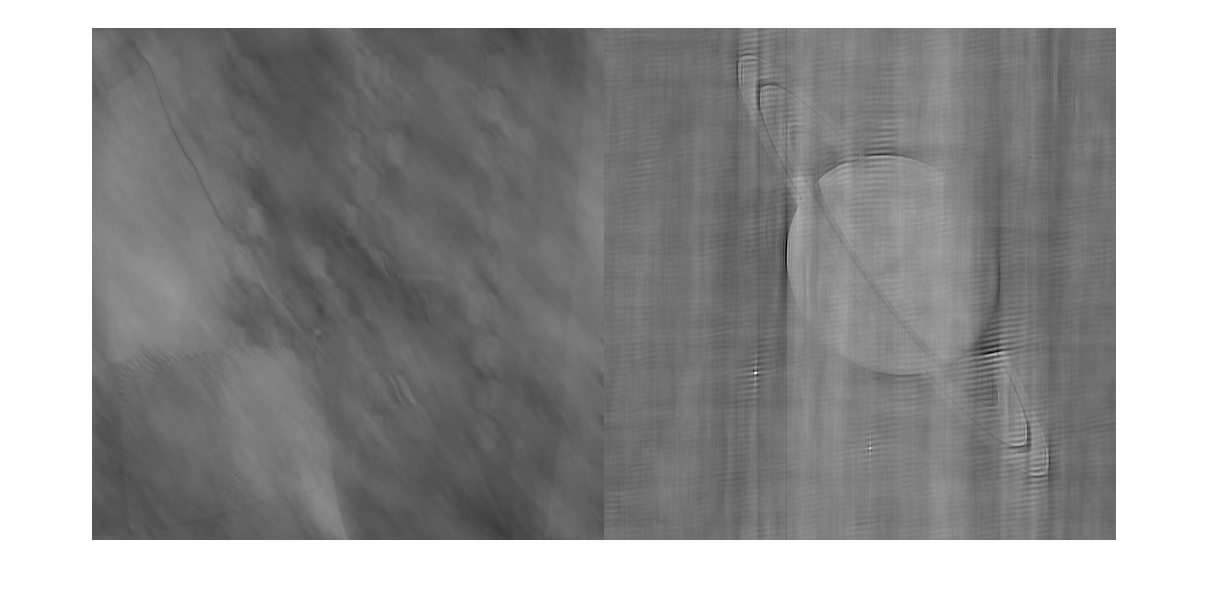
\includegraphics[height = 0.30\textheight]{10_1_12}
		\subcaption{Images dont les phases ont été échangées}
		\label{10_1_12}
	\end{subfigure}
	\caption{Echange de phase entre \textit{room.pgm} et \textit{saturn.pgm}}
	\label{10_1}
\end{figure}

\begin{figure}[H]
	\centering
	\begin{subfigure}[b]{\textwidth}
		\centering
		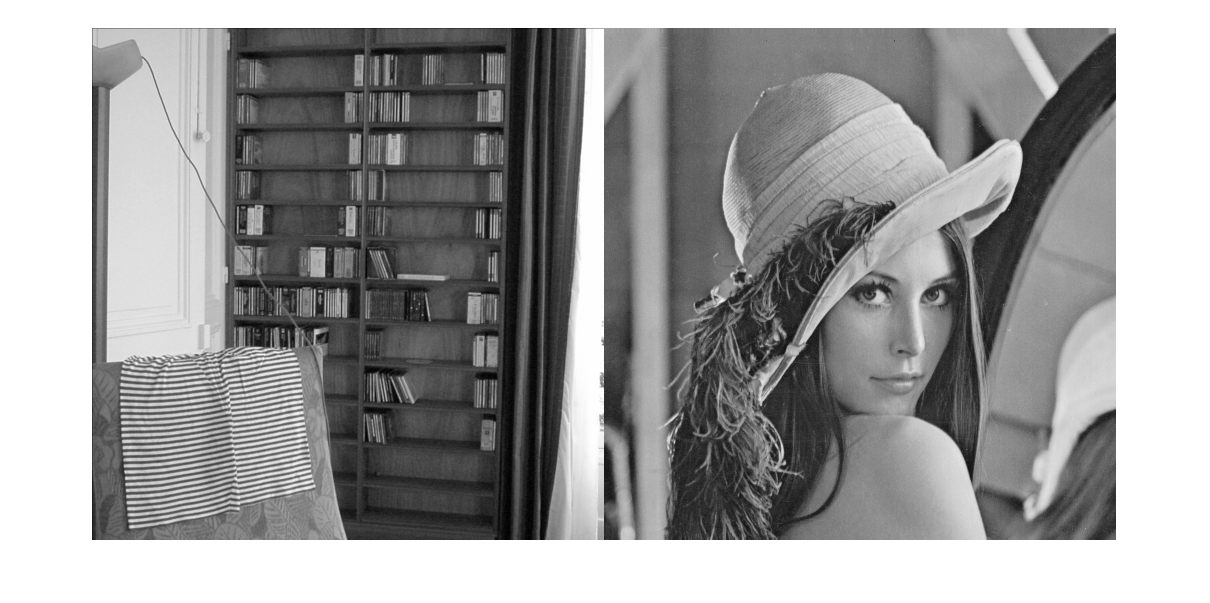
\includegraphics[height = 0.30\textheight]{10_1_21}
		\subcaption{Images initiales}
		\label{10_1_21}
	\end{subfigure}
	\vspace{2cm}
	\begin{subfigure}[b]{\textwidth}
		\centering
		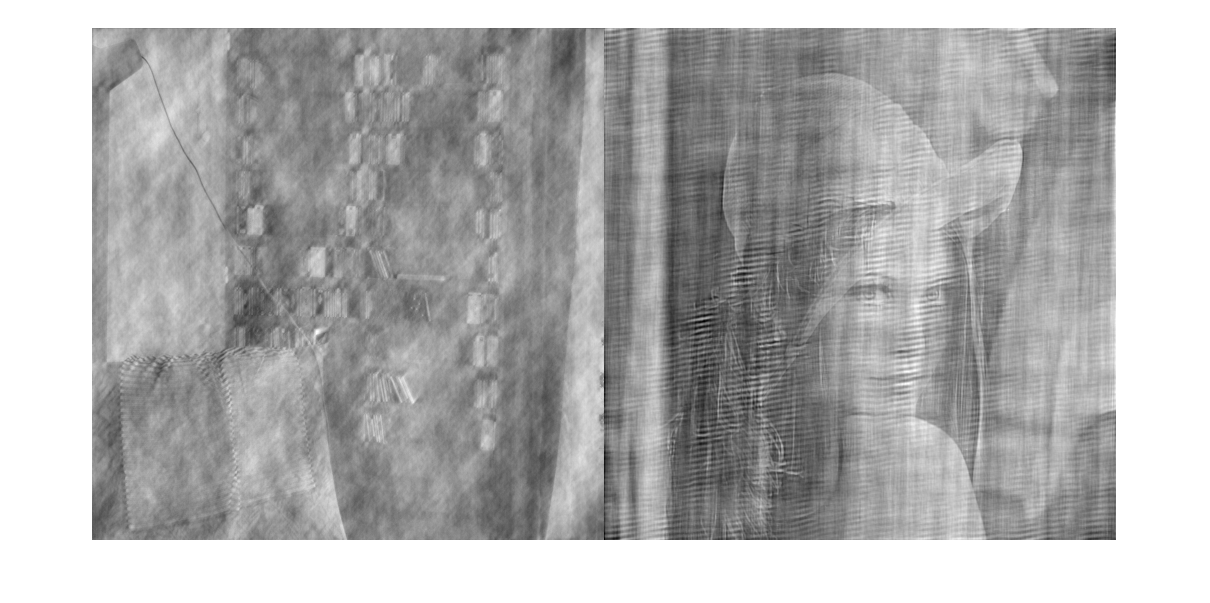
\includegraphics[height = 0.30\textheight]{10_1_22}
		\subcaption{Images dont les phases ont été échangées}
		\label{10_1_22}
	\end{subfigure}
	\caption{Echange de phase entre \textit{room.pgm} et \textit{lena.pgm}}
	\label{10_2}
\end{figure}

Deux exemples sont présentés en figures~\ref{10_1}~\ref{10_2}. On constate que toute l'information n'est pas contenue uniquement dans le module de la transformée de Fourier, puisqu'on appercoit, avec le module de \textit{saturne} et la phase de \textit{room}, les rayures du coussin, ainsi que la forme de la bibliothèque. De la même façon, on apperçoit aussi lena dans l'image où on garde le module de \textit{room} et on ajoute la phase de \textit{lena}. En revanche, on semble conserver mieux les objets quand on garde le module de la transformée de Fourier.

\subsection{Question 2}

\begin{figure}
	\centering
	\begin{subfigure}[b]{\textwidth}
		\centering
		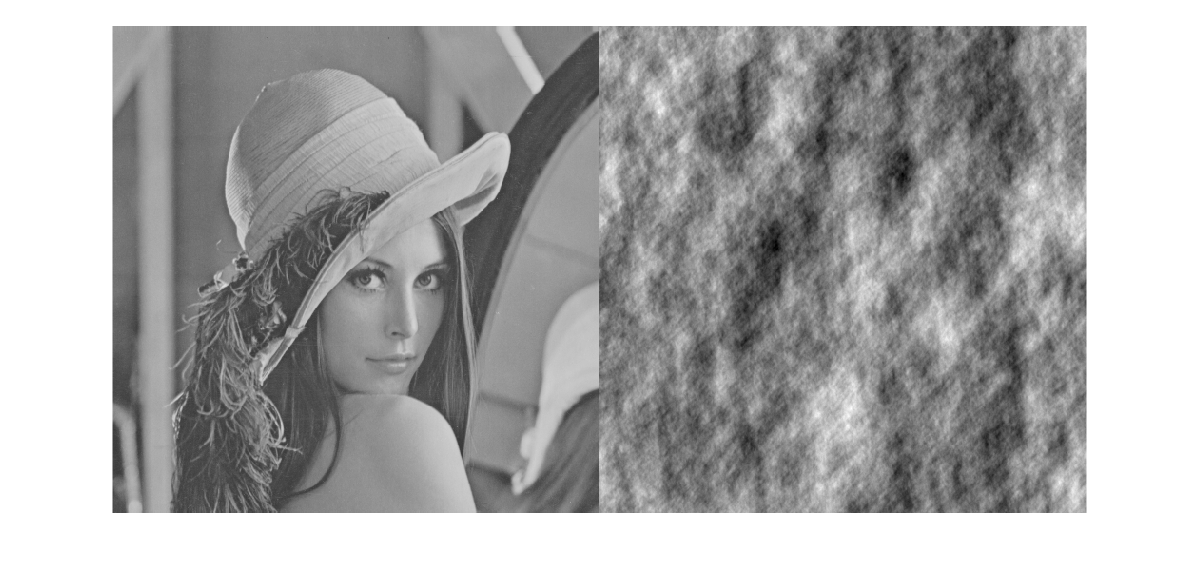
\includegraphics[height = 0.20\textheight]{10_2_lena}
		\subcaption{A partir de \textit{lena}}
		\label{10_2_lena}
	\end{subfigure}
	\begin{subfigure}[b]{\textwidth}
		\centering
		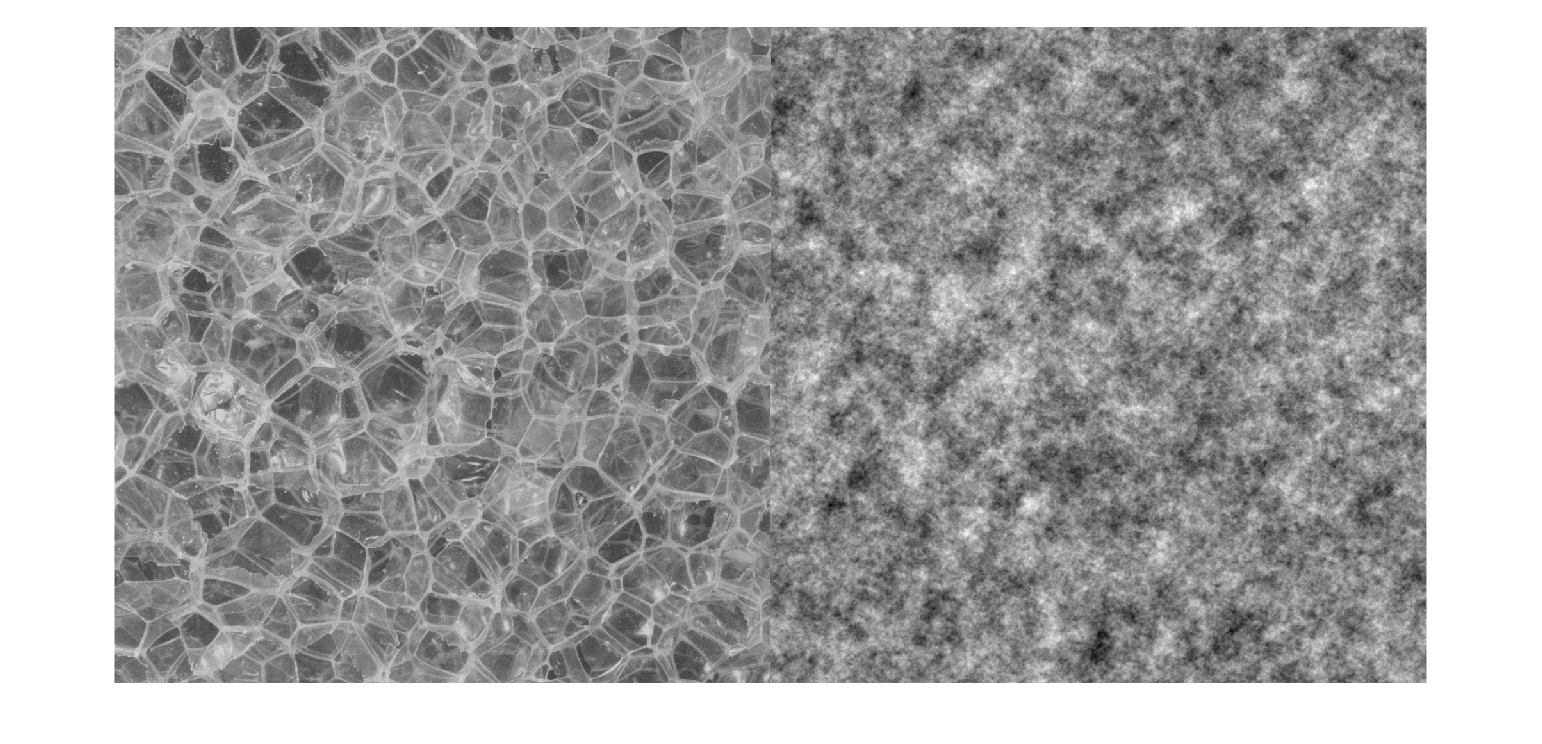
\includegraphics[height = 0.20\textheight]{10_2_bulles}
		\subcaption{A partir de bulles de plastique}
		\label{10_2_bulles}
	\end{subfigure}
	\begin{subfigure}[b]{\textwidth}
		\centering
		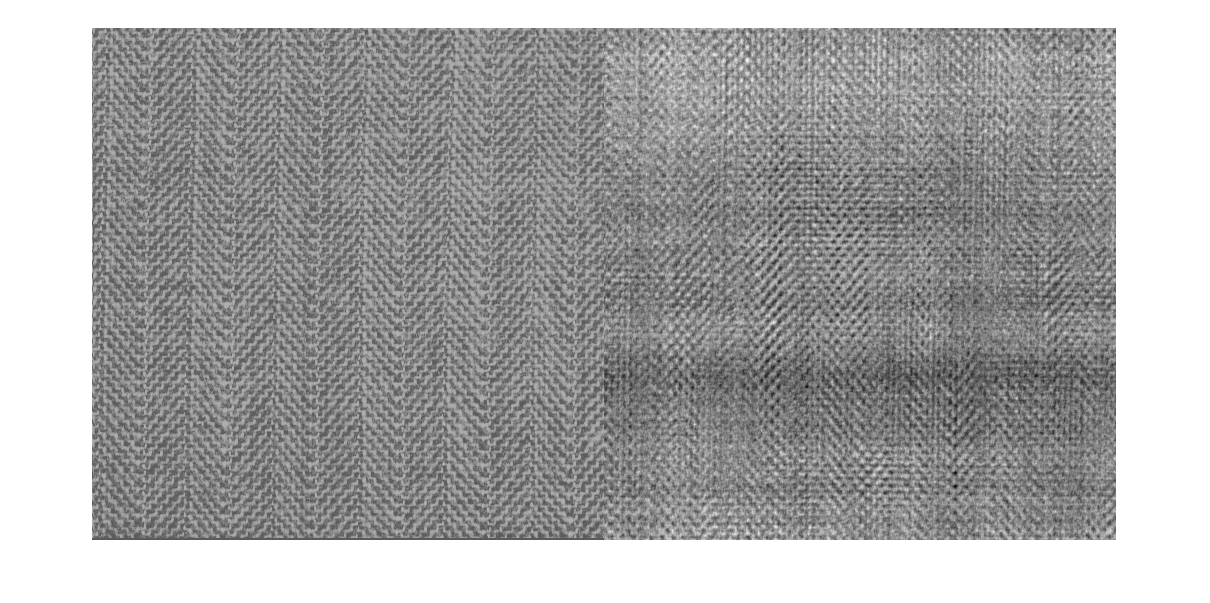
\includegraphics[height = 0.20\textheight]{10_2_tissu}
		\subcaption{A partir d'un tissu avec des motifs en chevrons}
		\label{10_2_tissu}
	\end{subfigure}
	\begin{subfigure}[b]{\textwidth}
		\centering
		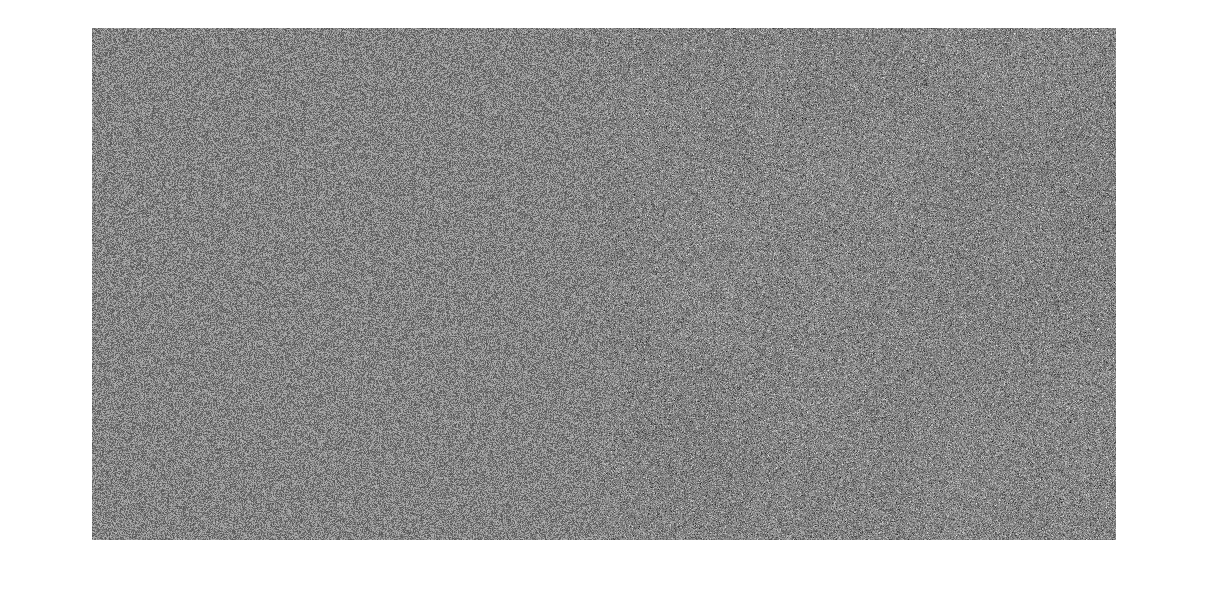
\includegraphics[height = 0.20\textheight]{10_2_noise}
		\subcaption{A partir de bruit blanc gaussien}
		\label{10_2_noise}
	\end{subfigure}
	\caption{Synthèse de texture à partir de la composante périodique : sur la colonne de gauche, l'image originale, sur la colonne de droite : l'image synthétisée}
	\label{10_2_textures}
\end{figure}

En figure~\ref{10_2_textures} sont présentées les synthèses d'images à phase aléatoire obtenues a partir d'images d'objets, en figure~\ref{10_2_lena}, et d'images de textures en figures~\ref{10_2_bulles}~\ref{10_2_tissu}~\ref{10_2_noise}. On constate que les microtextures sont celles le mieux reproduites, et c'était attendu car l'information spatiale contenue dans la phase est perdue à grande échelle par le fait de rendre la phase aléatoire. En particulier, en figure~\ref{10_2_textures}, on constate que les images synthétisées sont d'autant plus vraisemblables que le motif de texture initial est fin, avec pour limite le bruit blanc gaussien en figure~\ref{10_2_noise}.

En travaillant directement avec l'image, sans passer par sa composante périodique, on constate que près des bords (verticaux) de l'image, on retrouve majoritairement l'information de l'image initiale, comme observé en figure~\ref{10_2_aper}. Cela s'explique car la composante continue tue l'énergie le long des axes de la transformée de Fourier, qui n'est plus tuée si on ne considère plus uniquement cette composante continue. Ainsi, l'énergie du module de la transformée de Fourier prédomine toujours dans l'image synthétisée, comme on peut le constater dans la visualisation de la différence des transformée de Fourier de la composante périodique et de l'image initiale, présentée en figure~\ref{10_2_aper_fft}


\begin{figure}[H]
	\centering
	\begin{subfigure}[b]{\textwidth}
		\centering
		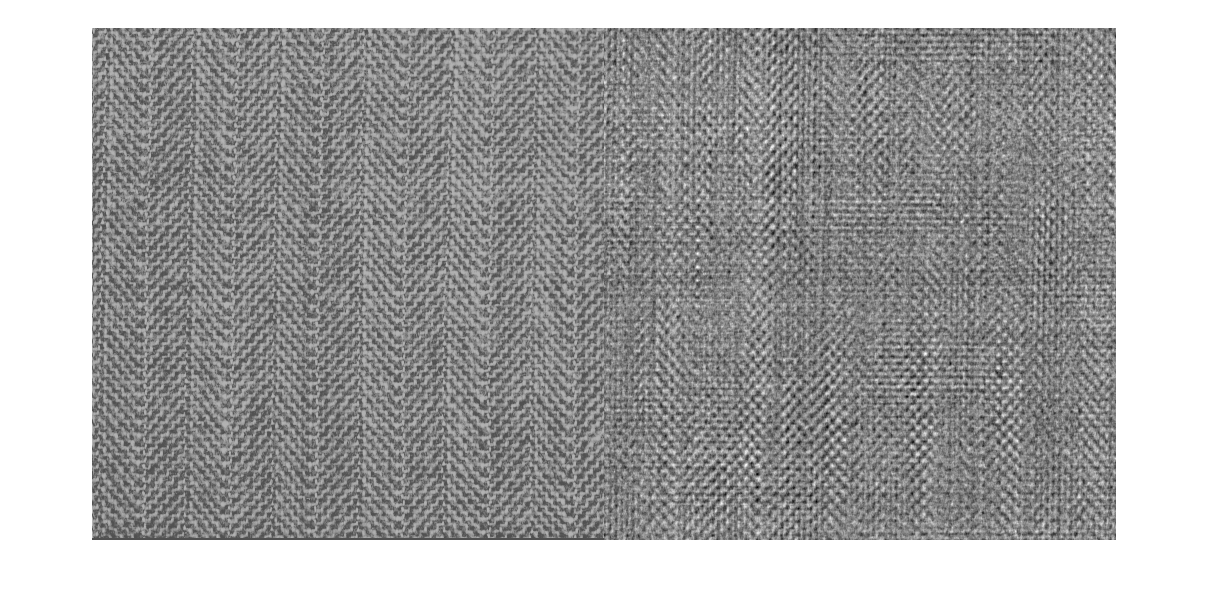
\includegraphics[width = 0.9\textwidth]{10_2_tissu_aper}
		\subcaption{A partir de bruit blanc gaussien}
		\label{10_2_aper_image}
	\end{subfigure}
	\begin{subfigure}[b]{\textwidth}
		\centering
		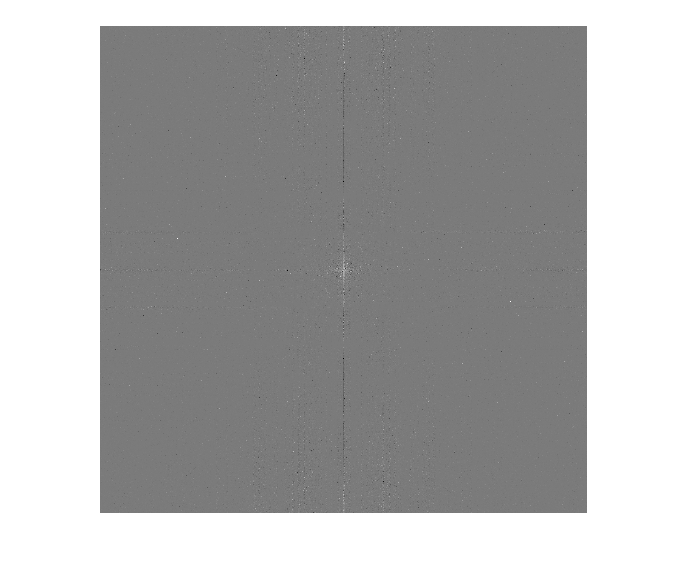
\includegraphics[width = 0.5\textwidth]{10_2_tissu_aper_fft}
		\subcaption{Tranformée de Fourier de l'image synthétisée à partir de la différence de la composante périodique et de l'image synthétisée à partir de l'image brute}
		\label{10_2_aper_fft}
	\end{subfigure}
	\caption{Synthèse de texture à partir de l'image initiale de la figure~\ref{10_2_tissu} sans extraire la composante continue}
	\label{10_2_aper}
\end{figure}

\subsection{Question 3}


\begin{figure}[H]
	\centering
	\begin{subfigure}[b]{\textwidth}
		\centering
		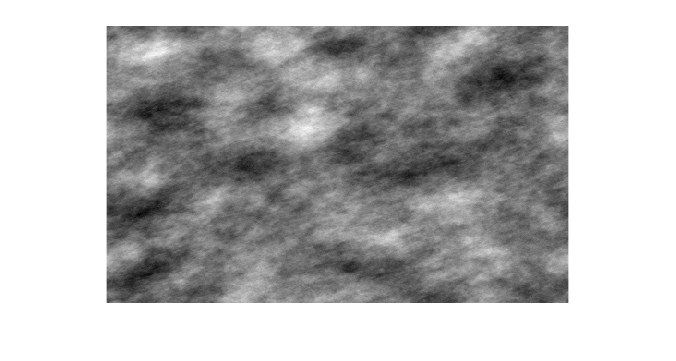
\includegraphics[width = 0.9\textwidth]{10_3_obj}
		\subcaption{Image \textit{texture} synthétisée}
		\label{10_3_11}
	\end{subfigure}
	\begin{subfigure}[b]{\textwidth}
		\centering
		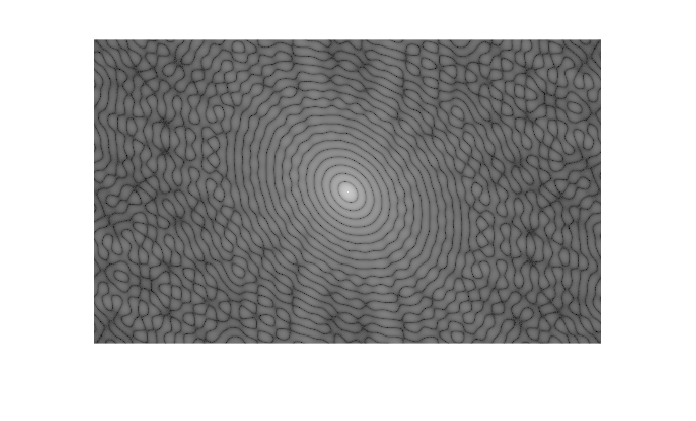
\includegraphics[width = 0.9\textwidth]{10_3_obj_fft}
		\subcaption{Tranformée de Fourier de \textit{texture}}
		\label{10_3_obj_fft}
	\end{subfigure}
	\caption{Visualisation de \textit{texture} et de sa tranformée de Fourier}
	\label{10_3_obj}
\end{figure}

En figure~\ref{10_3_obj} on peut visualiser l'image de texture synthétisée à partir d'une ellipse, ainsi que sa tranformée de Fourier. Le but est de retrouver les caractéristiques de l'ellipse à partir de laquelle a été synthétisée la figure~\ref{10_3_11} par ramdomisation de la phase. Il suffit donc de trouver l'ellipse dont la transformée de Fourier est présentée en figure~\ref{10_3_obj_fft}. Celle-ci est en fait la convolution d'une ellipse avec un sinus cardinal séparable à 2 dimensions, format des rebonds elliptiques permettant de déterminer l'axe principal de l'ellipse, comme étant perpendiculaire à l'axe principal de ces rebonds, c'est à dire que l'axe principal de l'ellipse initial est incliné de \(\frac{\pi}{4} \pm \pi\) par rapport à l'axe des abscisses. Les

\end{document}
